\documentclass[../../../main.tex]{subfiles}

\begin{document}

\chapter{[G] Projective Geometry}

Projective geometry, unlike euclidean geometry, relies on the
relationship between objects and their projections. One way I like to
think about it is the study of shades. There are  important topics
that cannot be solved without prior knowledge, so let's dive into it!

\section{Foundations}

Before we get into some important theorems and topics, lets discuss
some of its foundational properties to get the gut feeling for future
topics.

\begin{minipage}{0.48\textwidth}
\begin{figure}[H]
\centering
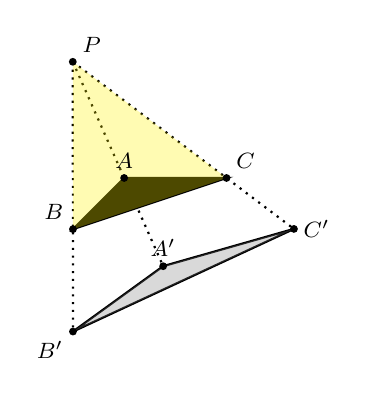
\begin{tikzpicture}[scale=0.13]
    \coordinate (A) at (5, 15);
    \coordinate (B) at (0, 10);
    \coordinate (C) at (15, 15);
    \coordinate (A') at (8.81, 6.384);
    \coordinate (B') at (0, 0);
    \coordinate (C') at (21.585, 10.024);
    \coordinate (P) at (-0.018, 26.349);
    \coordinate (G) at (-36.326, -26.326);
    \coordinate (I) at (39.052, 15);
    \coordinate (H) at (76.3, 35.433);

    \draw[thick] (A) -- (B) -- (C) -- (A);
    \draw[thick] (A') -- (B') -- (C') -- (A');

    \draw[thick, dotted] (P) -- (A');
    \draw[thick, dotted] (P) -- (B');
    \draw[thick, dotted] (P) -- (C');

    \fill[black] (A) -- (B) -- (C);
    \fill[yellow, opacity=0.3] (P) -- (B) -- (C);
    \fill[gray, opacity=0.3] (A') -- (B') -- (C');

    \foreach \n in {A, B, C, A', B', C', P}
    \node at (\n)[circle,fill,inner sep=1pt]{};

    \node[above] at (A) {\footnotesize $A$};
    \node[above left] at (B) {\footnotesize $B$};
    \node[above right] at (C) {\footnotesize $C$};
    \node[above] at (A') {\footnotesize $A'$};
    \node[below left] at (B') {\footnotesize $B'$};
    \node[right] at (C') {\footnotesize $C'$};
    \node[above right] at (P) {\footnotesize $P$};
\end{tikzpicture}
\caption{}
\label{fig:Desargues Theorem Figure 1}
\end{figure}
\end{minipage}
\hfill
\begin{minipage}{0.48\textwidth}
First, consider the two, not necessarily similar, triangles and a
point $P$. From the diagram on the left, we can think of it as having
a light source $P$ that shines $\triangle{ABC}$. There, we get our
outcome $\triangle{A'B'C'}$, and we say that $A', B', C'$ are
corresponding points of $A, B, C$ respectively. Similarly,
we could state that $\overline{A'B'}, \overline{B'C'},
\overline{C'A'}$ are
\end{minipage}

corresponding sides of $\overline{AB}, \overline{BC}, \overline{CA}$
respectively.

\subsection{Cross Ratio}

Cross ratio is a very important topic that lays foundations to many
contents that we are going to discuss from now so it is very important
to fully understand them! First, consider the following diagram
with four collinear points $A, B, C, D$.

\begin{figure}[H]
\centering
\begin{tikzpicture}[scale=1.5]
    \coordinate (A) at (0, 0);
    \coordinate (B) at (1, 0);
    \coordinate (C) at (2, 0);
    \coordinate (D) at (3, 0);

    \draw[thick] (A) -- (B);
    \draw[thick] (B) -- (C);
    \draw[thick] (C) -- (D);

    \draw[fill=BrickRed] (A) circle (0.05);
    \draw[fill=BrickRed] (B) circle (0.05);
    \draw[fill=BrickRed] (C) circle (0.05);
    \draw[fill=BrickRed] (D) circle (0.05);

    \node[below] at (A) {\footnotesize $A$};
    \node[below] at (B) {\footnotesize $B$};
    \node[below] at (C) {\footnotesize $C$};
    \node[below] at (D) {\footnotesize $D$};

    \node[below] at ($(A)!0.5!(B)$) {\footnotesize $x$};
    \node[below] at ($(B)!0.5!(C)$) {\footnotesize $y$};
    \node[below] at ($(C)!0.5!(D)$) {\footnotesize $z$};
\end{tikzpicture}
\end{figure}

From the diagram above, we could define a new term.

\begin{important}
The \textbf{cross-ratio} of $A, B, C, D$ is defined as the following.
\[
(A, B; C, D) = \frac{(x + y) (y + z)}{y (x + y + z)}
\]
\end{important}

This is very important because if we project these points with
respect to another line by a point say $P$, then the cross ratio
of the resulting points is the same as the original value.
Consider the following diagram for an illustration.

\begin{figure}[H]
\centering
\begin{tikzpicture}[scale=0.8]
    \coordinate (P) at (4.5, 6);
    \coordinate (A) at (3, 4);
    \coordinate (B) at (4,4);
    \coordinate (C) at (5.5,4);
    \coordinate (D) at (6.75,4);
    \coordinate (A') at (0, 0);
    \coordinate (B') at (3.176470588235294,0.7058823529411765);
    \coordinate (C') at (6.75,1.5);
    \coordinate (D') at (9, 2);
    \coordinate (A'') at (2.051470588235294,8.176470588235293);
    \coordinate (B'') at (3.659090909090909,7.681818181818182);
    \coordinate (C'') at (4.830357142857143,7.321428571428571);
    \coordinate (D'') at (5.3671875,7.15625);

    \draw[thick] (A) -- (D);
    \draw[thick] (A') -- (D');
    \draw[thick] (A'') -- (D'');
    
    \draw[thick, dotted] (P) -- (A');
    \draw[thick, dotted] (P) -- (A'');
    \draw[thick, dotted] (P) -- (B');
    \draw[thick, dotted] (P) -- (B'');
    \draw[thick, dotted] (P) -- (C');
    \draw[thick, dotted] (P) -- (C'');
    \draw[thick, dotted] (P) -- (D');
    \draw[thick, dotted] (P) -- (D'');

    \draw[fill=black] (A) circle (0.05);
    \draw[fill=black] (B) circle (0.05);
    \draw[fill=black] (C) circle (0.05);
    \draw[fill=black] (D) circle (0.05);
    \draw[fill=BrickRed] (A') circle (0.05);
    \draw[fill=BrickRed] (B') circle (0.05);
    \draw[fill=BrickRed] (C') circle (0.05);
    \draw[fill=BrickRed] (D') circle (0.05);
    \draw[fill=RoyalPurple] (A'') circle (0.05);
    \draw[fill=RoyalPurple] (B'') circle (0.05);
    \draw[fill=RoyalPurple] (C'') circle (0.05);
    \draw[fill=RoyalPurple] (D'') circle (0.05);

    \node[left] at (A) {\footnotesize $A$};
    \node[below] at (B) {\footnotesize $B$};
    \node[below] at (C) {\footnotesize $C$};
    \node[right] at (D) {\footnotesize $D$};
    \node[below] at (A') {\footnotesize $A'$};
    \node[below] at (B') {\footnotesize $B'$};
    \node[below] at (C') {\footnotesize $C'$};
    \node[below] at (D') {\footnotesize $D'$};
    \node[left] at (A'') {\footnotesize $A''$};
    \node[above] at (B'') {\footnotesize $B''$};
    \node[above] at (C'') {\footnotesize $C''$};
    \node[right] at (D'') {\footnotesize $D''$};

    \node[below] at ($(A)!0.5!(B)$) {\footnotesize $x$};
    \node[below] at ($(B)!0.5!(C)$) {\footnotesize $y$};
    \node[below] at ($(C)!0.5!(D)$) {\footnotesize $z$};
    \node[below] at ($(A')!0.5!(B')$) {\footnotesize $x'$};
    \node[below] at ($(B')!0.5!(C')$) {\footnotesize $y'$};
    \node[below] at ($(C')!0.5!(D')$) {\footnotesize $z'$};
    \node[above] at ($(A'')!0.5!(B'')$) {\footnotesize $x''$};
    \node[above] at ($(B'')!0.5!(C'')$) {\footnotesize $y''$};
    \node[above] at ($(C'')!0.5!(D'')$) {\footnotesize $z''$};

    \pic[draw,"$\alpha$",angle radius=3mm,angle eccentricity=1.6]
        {angle=A--P--B};
    \pic[draw,"$\beta$",angle radius=4mm,angle eccentricity=1.6]
        {angle=B--P--C};
    \pic[draw,"$\gamma$",angle radius=5mm,angle eccentricity=1.6]
        {angle=C--P--D};
\end{tikzpicture}
\end{figure}

In this diagram, we can see that the following equation holds.
\[
(A, B; C, D) = (A', B'; C', D') = (A'', B''; C'', D'')
\]
To prove this, let's use length area ratio. Consider the following
equations.
\begin{align*}
    (A, B; C, D)
    &= \frac{(x + y)(y + z)}{y (x + y + z)}
    = \frac{ [\triangle{PAC}] \cdot [\triangle{PBD}] }
        { [\triangle{PBC}] \cdot [\triangle{PAD}] } \\
    &= \frac{
        PA \cdot PC \cdot \sin(\alpha + \beta) \cdot
        PB \cdot PD \cdot \sin(\beta + \gamma)
    }{
        PB \cdot PC \cdot \sin\beta \cdot
        PA \cdot PD \cdot \sin(\alpha + \beta + \gamma)
    } \\
    &= \frac{ \sin(\alpha + \beta) \cdot \sin(\beta + \gamma) }
        { \sin\beta \cdot \sin(\alpha + \beta + \gamma) } \\
    &= \frac{ [\triangle{PA'C'}] \cdot [\triangle{PB'D'}] }
        { [\triangle{PB'C'}] \cdot [\triangle{PA'D'}] }
    = (A', B'; C', D')
\end{align*}
The same argument applies for the top one, or you could just think
of it as the rotated version.

Continuing with this, we can implement this idea to four points
on a circle. I think this is one of the foundational topic that
could act as the breakthrough.

\begin{figure}[H]
\centering
\begin{tikzpicture}[scale=0.9]
    \coordinate (P) at (0,3);
    \coordinate (A) at (-2.4484583429038547,-1.7335085067759288);
    \coordinate (B) at (-0.7901879601928523,-2.8940634042063174);
    \coordinate (C) at (1.3678086197709374,-2.6700373742103913);
    \coordinate (D) at (2.3685924325386085,-1.841132773191776);
    \coordinate (A') at (-3.620825519969496,-4);
    \coordinate (B') at (-0.9384554155631452,-4);
    \coordinate (C') at (1.6886414862000672,-4);
    \coordinate (D') at (3.4248486469085027,-4);

    \draw (0, 0) circle (3);
    \draw[thick] (A) -- (B) -- (C) -- (D) -- cycle;
    \draw[thick] (A') -- (D');
    
    \draw[thick, dotted] (P) -- (A');
    \draw[thick, dotted] (P) -- (B');
    \draw[thick, dotted] (P) -- (C');
    \draw[thick, dotted] (P) -- (D');

    \draw[fill=black] (A) circle (0.05);
    \draw[fill=black] (B) circle (0.05);
    \draw[fill=black] (C) circle (0.05);
    \draw[fill=black] (D) circle (0.05);
    \draw[fill=BrickRed] (A') circle (0.05);
    \draw[fill=BrickRed] (B') circle (0.05);
    \draw[fill=BrickRed] (C') circle (0.05);
    \draw[fill=BrickRed] (D') circle (0.05);

    \node[above] at (P) {\footnotesize $P$};
    \node[left] at (A) {\footnotesize $A$};
    \node[below] at (B) {\footnotesize $B$};
    \node[below] at (C) {\footnotesize $C$};
    \node[right] at (D) {\footnotesize $D$};
    \node[below] at (A') {\footnotesize $A'$};
    \node[below] at (B') {\footnotesize $B'$};
    \node[below] at (C') {\footnotesize $C'$};
    \node[below] at (D') {\footnotesize $D'$};

    \node[below] at ($(A)!0.5!(B)$) {\footnotesize $x$};
    \node[below] at ($(B)!0.5!(C)$) {\footnotesize $y$};
    \node[below] at ($(C)!0.5!(D)$) {\footnotesize $z$};
    \node[below] at ($(A')!0.5!(B')$) {\footnotesize $x'$};
    \node[below] at ($(B')!0.5!(C')$) {\footnotesize $y'$};
    \node[below] at ($(C')!0.5!(D')$) {\footnotesize $z'$};

    \pic[draw,"$\alpha$",angle radius=6mm,angle eccentricity=1.6]
        {angle=A--P--B};
    \pic[draw,"$\beta$",angle radius=7mm,angle eccentricity=1.6]
        {angle=B--P--C};
    \pic[draw,"$\gamma$",angle radius=8mm,angle eccentricity=1.6]
        {angle=C--P--D};
\end{tikzpicture}
\end{figure}

From this diagram, we will use the Law of Sines to show that
$(A, B; C, D) \linebreak = (A', B'; C', D')$. First, notice that
$(A', B'; C', D') = \frac{
    \sin(\alpha + \beta) \cdot \sin(\beta + \gamma)
}{ \sin\beta \cdot \sin(\alpha + \beta + \gamma) }$ from our previous
observation. Moreover, the following equations hold.
\begin{align*}
    \frac{
        \sin(\alpha + \beta) \cdot \sin(\beta + \gamma)
    }{ \sin\beta \cdot \sin(\alpha + \beta + \gamma) }
    &= 
    \frac{
        \frac{\sin(\alpha + \beta)}{AC} \cdot
        \frac{\sin(\beta + \gamma)}{BD}
    }{
        \frac{\sin\beta}{BC} \cdot
        \frac{\sin(\alpha + \beta + \gamma)}{AD}
    }
    \cdot \frac{AC \cdot BD}{BC \cdot AD} \\
    &= \frac{
        \frac{\sin\angle{PDA}}{PA} \cdot
        \frac{\sin\angle{PAD}}{PD}
    }{
        \frac{\sin\alpha}{AB} \cdot
        \frac{\sin\angle{PAD}}{PD}
    }
    \cdot \frac{AC \cdot BD}{BC \cdot AD} \\
    &= \frac{ \frac{\sin\angle{PDA}}{PA} }{ \frac{\sin\alpha}{AB} }
        \cdot \frac{AC \cdot BD}{BC \cdot AD} \\
    &= \frac{AC \cdot BD}{BC \cdot AD} = (A, B; C, D)
\end{align*}
Therefore, the cross ratio is consistent if $A, B, C, D$ lies on a
circle any they are projected to a line from another point on the
circle. Continuing, we can define a new term.

\begin{definition}{}{}
A \textbf{harmonic quadrilateral} $ABCD$ is a cyclic quadrilateral
such that $(A, B; C, D) = -1$.
\end{definition}

Another way of understanding harmonic quadrilateral is a cyclic
quadrilateral with same product of the lengths of opposite edges
are equal. It is pretty obvious using Ptolemy and the definition
of cross ratio.

Next one is even more interesting. It is about projection of of a
cyclic quadrilateral on to the inscribing circle.

\begin{important}
In the diagram below, $(A, B; C, D) = (A', B'; C', D')$.
\end{important}

\begin{figure}[H]
\centering
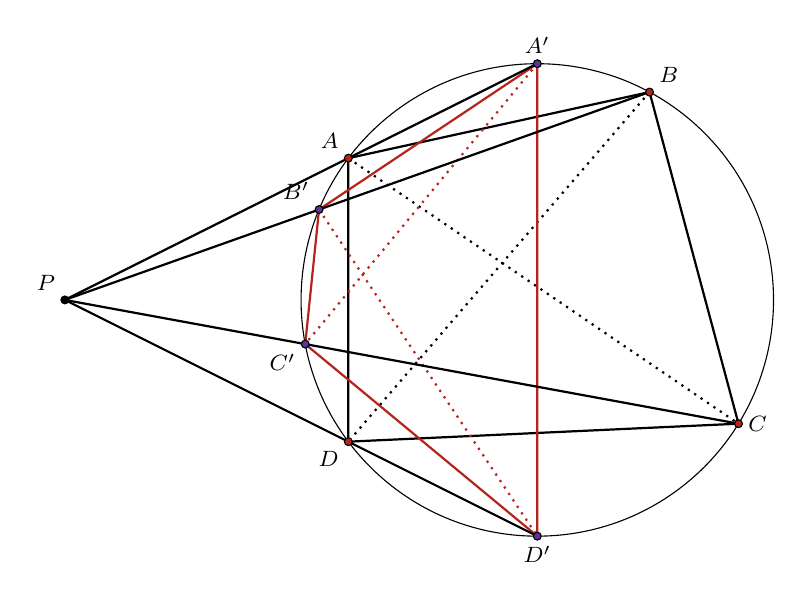
\begin{tikzpicture}
    \coordinate (O) at (0, 0);
    \coordinate (A) at (-2.4,1.8);
    \coordinate (B) at (1.425022379602948,2.6399453058028968);
    \coordinate (C) at (2.555323047845728,-1.5717264778416182);
    \coordinate (D) at (-2.4,-1.8);
    \coordinate (A') at (0,3);
    \coordinate (B') at (-2.771743360965249,1.1477973431512487);
    \coordinate (C') at (-2.947106958424652,-0.5608570010305624);
    \coordinate (D') at (0,-3); 
    \coordinate (P) at (-6,0);

    \draw (0, 0) circle (3);
    \draw[thick] (A) -- (B) -- (C) -- (D) -- cycle;
    \draw[thick, dotted] (A) -- (C);
    \draw[thick, dotted] (B) -- (D);
    \draw[thick, BrickRed] (A') -- (B') -- (C') -- (D') -- cycle;
    \draw[thick, BrickRed, dotted] (A') -- (C');
    \draw[thick, BrickRed, dotted] (B') -- (D');
    \draw[thick] (P) -- (A');
    \draw[thick] (P) -- (B);
    \draw[thick] (P) -- (C);
    \draw[thick] (P) -- (D');

    \draw[fill=black] (P) circle (0.05);
    \draw[fill=BrickRed] (A) circle (0.05);
    \draw[fill=BrickRed] (B) circle (0.05);
    \draw[fill=BrickRed] (C) circle (0.05);
    \draw[fill=BrickRed] (D) circle (0.05);
    \draw[fill=RoyalPurple] (A') circle (0.05);
    \draw[fill=RoyalPurple] (B') circle (0.05);
    \draw[fill=RoyalPurple] (C') circle (0.05);
    \draw[fill=RoyalPurple] (D') circle (0.05);

    \node[above left] at (P) {\footnotesize $P$};
    \node[above left] at (A) {\footnotesize $A$};
    \node[above right] at (B) {\footnotesize $B$};
    \node[right] at (C) {\footnotesize $C$};
    \node[below left] at (D) {\footnotesize $D$};
    \node[above] at (A') {\footnotesize $A'$};
    \node[above left] at (B') {\footnotesize $B'$};
    \node[below left] at (C') {\footnotesize $C'$};
    \node[below] at (D') {\footnotesize $D'$};
\end{tikzpicture}
\end{figure}

To prove this, we can use similar triangles. First, through simple
angle chasing, it is evident that the following triangles are
similar through AA similarity.
\begin{align*}
    \triangle{PAC} &\sim \triangle{PC'A'} \\
    \triangle{PDB} &\sim \triangle{PB'D'} \\
    \triangle{PAD} &\sim \triangle{PD'A'} \\
    \triangle{PB'C'} &\sim \triangle{PCB}
\end{align*}
Using the length ratio of the similar triangles, we obtain following
equations.
\begin{align*}
    \frac{AC}{A'C'} &= \frac{PA}{PC'} = \frac{PC}{PA'} \\
    \frac{BD}{B'D'} &= \frac{PD}{PB'} = \frac{PB}{PD'} \\
    \frac{A'D'}{AD} &= \frac{PD'}{PA} = \frac{PA'}{PD} \\
    \frac{B'C'}{BC} &= \frac{PB'}{PC} = \frac{PC'}{PB}
\end{align*}
Multiplying the equations,
\begin{align*}
    &\quad\ \frac{AC}{A'C'} \cdot \frac{BD}{B'D'} \cdot \frac{A'D'}{AD}
        \cdot \frac{B'C'}{BC} \\
    &= \sqrt{
        \frac{PA}{PC'} \cdot \frac{PC}{PA'} \cdot
        \frac{PD}{PB'} \cdot \frac{PB}{PD'} \cdot
        \frac{PD'}{PA} \cdot \frac{PA'}{PD} \cdot
        \frac{PB'}{PC} \cdot \frac{PC'}{PB}
    }
    = 1
\end{align*}
is obtained with $\frac{AC \cdot BD}{AD \cdot BC} =
\frac{A'C' \cdot B'D'}{A'D' \cdot B'C'}$, and $(A, B; C, D) =
(A', B'; C', D')$.

Before we wrap-up this section, consider the following theorem.
This theorem comes especially handy when you have to draw a symmedian
because many olympiads don't allow protractor.

\begin{theorem}{}{}
Given a harmonic quadrilateral $ABCD$, $BD$ is the symmedian from $B$
of $\triangle{ABC}$.
\end{theorem}
\begin{proof}
First, notice that by Theorem \ref{theo:Symmedian and Lengths},
it suffices to show that $\frac{AK}{CK} = \frac{BA^2}{BC^2}$.
Consider the following equations.
\begin{align*}
    \frac{AK}{CK}
    &= \frac{[\triangle{ABD}}{[\triangle{BCD}]}
    = \frac{
        \frac{1}{2} AB \cdot AD \cdot \sin\angle{BAD}
    }{
        \frac{1}{2} BC \cdot CD \cdot \sin\angle{BCD}
    } \\
    &= \frac{AB \cdot AD}{BC \cdot CD}
    = \frac{AB}{BC} \cdot \frac{AB}{BC}
    = \frac{BA^2}{BC^2}
\end{align*}
Therefore, the theorem holds.
\end{proof}

With these concepts in mind, let's discuss some fundamental theorems
in projective geometry.

\end{document}


